\documentclass{beamer}

\usepackage{listings}
\usepackage{xcolor}
\usepackage{graphicx}

\definecolor{codegreen}{rgb}{0,0.6,0}
\definecolor{codegray}{rgb}{0.5,0.5,0.5}
\definecolor{codepurple}{rgb}{0.58,0,0.82}
\definecolor{backcolour}{rgb}{0.95,0.95,0.92}

\lstdefinestyle{mystyle}{
    backgroundcolor=\color{backcolour},   
    commentstyle=\color{codegreen},
    keywordstyle=\color{magenta},
    numberstyle=\tiny\color{codegray},
    stringstyle=\color{codepurple},
    basicstyle=\ttfamily\footnotesize,
    breakatwhitespace=false,         
    breaklines=true,                 
    captionpos=b,                    
    keepspaces=true,                 
    numbers=left,                    
    numbersep=5pt,                  
    showspaces=false,                
    showstringspaces=false,
    showtabs=false,                  
    tabsize=2
}

\lstset{style=mystyle}

%Information to be included in the title page:
\title{Low Level AVR}
\subtitle{Arduino? Nein danke!}
\author{Felix Queißner}
\institute{shackspace}
\date{2020}

\begin{document}

\frame{\titlepage}

\begin{frame}
\frametitle{Wer bin ich?}
\begin{itemize}
\item Felix „xq“ Queißner
\item Baujahr 1993
\item Mit 12 angefangen, zu programmieren
\item Mit 13 angefangen, Elektronik zu basteln
\item Mache gerne Dinge mit Code und alten Computern
\end{itemize}
\end{frame}

\begin{frame}
\frametitle{Worum geht's?}
\begin{itemize}
\item Grundlagenwissen AVR-Programmierung vermitteln
\item „Wie komme ich klar, wenn es mit der Arduino-IDE nicht mehr weiter geht?“
\item „Awareness schaffen“ für Code Bloat
\item \textbf{Nicht:} AVR/Arduino löten
\item \textbf{Nicht:} C programmieren lernen
\end{itemize}
\end{frame}

\begin{frame}
\frametitle{Outline}
\begin{enumerate}
\item Teaser
\item The Arduino way
\item Zum Ziel in vier Schritten
  \begin{enumerate}
  \item Dokumentation lesen
  \item Code schreiben
  \item Compilen \& Linken
  \item Flashen
  \end{enumerate}
\item Fazit
\item Wie geht's weiter?
\end{enumerate}
\end{frame}

\begin{frame}
\frametitle{Wie kommen wir von hier …}
\lstinputlisting[language=C]{bad-code.c}
\end{frame}

\begin{frame}
\frametitle{… nach da?}
\lstinputlisting[language=C]{good-code.c}
\end{frame}

\begin{frame}
\frametitle{The Arduino way}
\begin{itemize}
\item Schnell von „Idee“ zu „Es blinkt schon mal was“ kommen
\item Single-Click-Solution
\item Mit was man genau arbeitet ist eigentlich egal, es erfüllt alles den gleichen Zweck 
\end{itemize}
\end{frame}

\begin{frame}
\frametitle{Blink}
\begin{itemize}
\item Lässt eine LED mit \(\frac{1}{2}\) Hertz blinken
\item Benutzt \lstinline[language=C]{setup()} und \lstinline[language=C]{loop()}
\end{itemize}
\lstinputlisting[language=C]{blink.ino}
\end{frame}

\begin{frame}
\frametitle{Serial}
\begin{itemize}
\item Gibt \lstinline[language=C]{"Hello, World!"} auf der Konsole aus
\item Spiegelt anschließend die Texteingabe zurück
\item Benutzt \lstinline[language=C]{setup()} und \lstinline[language=C]{loop()}
\item Benutzt \lstinline[language=C]{Serial.*}
\end{itemize}
\lstinputlisting[language=C]{serial.ino}
\end{frame}

\begin{frame}
\frametitle{Pro/Contra Arduino}

\textbf{Pro:}
\begin{itemize}
\item Man kommt schnell zum Ziel
\item Zugrunde liegened Hardware ist schnell ausgetauscht
\item Es gibt viele Beispiele für die Arduino-Welt
\item „Batterien inklusive“
\end{itemize}

\textbf{Contra:}
\begin{itemize}
\item Es passiert sehr viel \textit{Magie}
\item Arduino-Programme sind „fett und träge“
\item Wir haben keine wirkliche Kontrolle über das Programm
\end{itemize}
  
\end{frame}

\begin{frame}
\frametitle{In vier Schritten zum Ziel}
\begin{enumerate}
\item Dokumentation lesen
\item Code schreiben
\item Compilen \& Linken
\item Flashen
\end{enumerate}
\end{frame}

\begin{frame}
\frametitle{Warum tun wir uns das an?}
\begin{itemize}
\item Programme werden kleiner
\item Programme werden schneller
\item Wir können die Hardware voll ausnutzen
\end{itemize}
\end{frame}

\begin{frame}
\frametitle{Schritt 1: Dokumentation lesen}

\textbf{Welche Dokumente brauchen wir?}
\begin{itemize}
\item Schaltplan
\item Datenblatt
\end{itemize}
\end{frame}

\begin{frame}
\frametitle{Schaltplan}
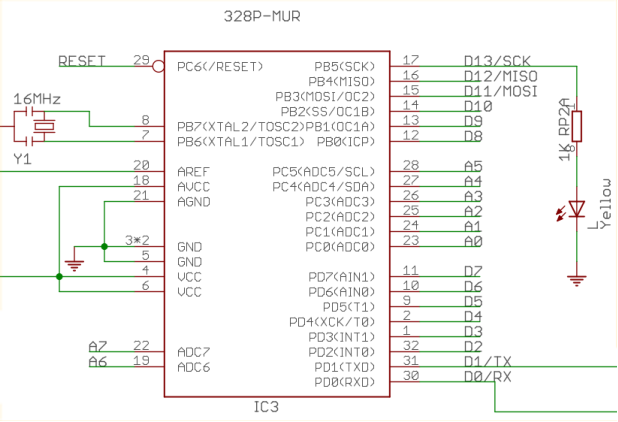
\includegraphics{schematic.pdf}
\end{frame}

% PC6 ist Reset, aber auch I/O!

\begin{frame}
\frametitle{Schaltplan}
\begin{itemize}
\item \textit{Ground Truth} für Pinbelegungen
\item Zeigt uns, wie die Hardware funktioniert
\item Offenbart manchmal undokumentierte Möglichkeiten
\end{itemize}


\end{frame}


% D6, D7 können als Input für den Analog-Komparator dienen!
% D2, D3 können externe Interrupts!

\begin{frame}
\frametitle{Datenblatt}
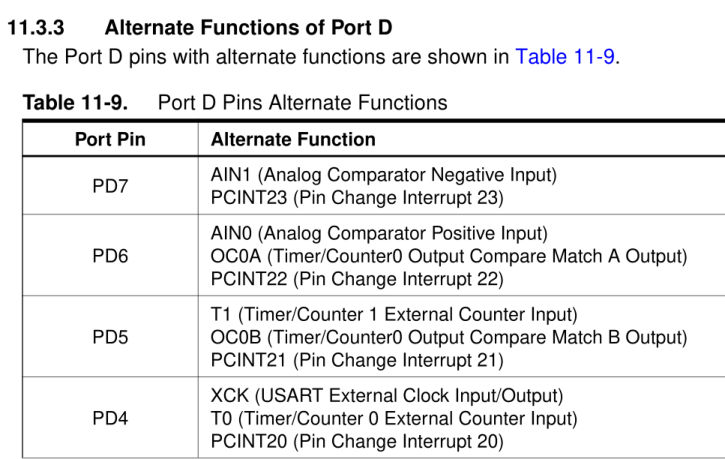
\includegraphics{datasheet.pdf}
\end{frame}

\begin{frame}
\frametitle{Datenblatt}
\begin{itemize}
\item \textit{Ground Truth} für Hardware-Funktionalität
\item Zeigt uns, wie der Microcontroller funktioniert
\item Hilfreich: Doppelfunktionen für Pin-Belegungen
\end{itemize}

\end{frame}

\begin{frame}
\frametitle{Schritt 2: Code schreiben}

\textbf{Allgemein:}
\begin{itemize}
\item C ist die primäre Embedded-Programmiersprache
\item C++, Basic, Pascal, Zig, Rust, … sind auf AVR ebenfalls verfügbar
\item Dynamische Speicherverwaltung wird selten benötigt
\end{itemize}

\textbf{Hands on:}
\begin{enumerate}
\item Code
\item Datenblatt verwenden
\item Komplexer Hardware-Init
\item Interrupt
\end{enumerate}
\end{frame}

\begin{frame}
\frametitle{Hands on: Code (Blink 1)}
\lstinputlisting[language=C]{blink1.c}
\end{frame}

\begin{frame}
\frametitle{Hands on: Datenblatt (Blink 2)}
\lstinputlisting[language=C]{blink2.c}
\end{frame}

\begin{frame}
\frametitle{Hands on: Hardware-Init (UART 1)}
\lstinputlisting[language=C]{uart1.c}
\end{frame}

\begin{frame}
\frametitle{Hands on: Interrupts (UART 2)}
\lstinputlisting[language=C]{uart2.c}
\end{frame}

\begin{frame}
\frametitle{Schritt 3: Compilen \& Linken}
\begin{itemize}
\item Was ist ein
    \begin{itemize}
    \item Compiler?
    \item Linker?
    \item Bibliothek?
    \item Makefile?
    \end{itemize}
\item Dateiformate
\item Tools
\end{itemize}
\end{frame}

\begin{frame}
\frametitle{Was ist ein Compiler?}
\begin{itemize}
\item Übersetzt Quellcode in Maschinensprache
\item Gibt „Object Files“ aus
\item Kann verschiedene Optimierungen durchführen
\item 
\end{itemize}
\lstinputlisting[language=C]{compile.sh}
\end{frame}

\begin{frame}
\frametitle{Was ist ein Linker?}
\begin{itemize}
\item Verknüpft „Object Files“
\item Weißt allen Dingen Adressen zu
\item Sortiert Objekte im Speicher
\item Bindet Bibliotheken ein
\item Ist konfigurierbar (Linkerscript)
\end{itemize}
\lstinputlisting[language=C]{link.sh}
\end{frame}

\begin{frame}
\frametitle{Was ist eine Bibliothek?}
\textbf{Grundlegend:}
\begin{itemize}
\item Sammlung von Funktionalität
\item Erlaubt Wiederverwendung von Code
\end{itemize}

\textbf{Statische Bibliothek:}
\begin{itemize}
\item Eine Sammlung von vorcompilierten Object Files
\item Keine Laufzeitkosten
\item Kann mit der richtigen Technik sogar nachträglich optimiert werden
\end{itemize}
\textbf{Dynamische Bibliothek:}
\begin{itemize}
\item Wird zu Programmstart in unsere ausführbare Datei geladen und gelinkt
\item Im Embedded-Bereich quasi nie eingesetzt
\item Konzept auf AVR unmöglich umzusetzen
\end{itemize}
\end{frame}

\begin{frame}
\frametitle{Was ist ein Makefile?}
\textbf{Wofür ein Buildsystem?}
\begin{itemize}
\item Viele wiederkehrende Tasks beim Entwickeln
\item Bedingtes Ausführen von Tasks
\item Bequeme Bedienung
\end{itemize}

\textbf{GNU Make:}
\begin{itemize}
\item Einfach zu bedienen
\item \lstinline{Makefile} enthält Regeln zum Ausführen von Befehlen
\item Tracking von Abhängigkeiten über Schreibdatum
\item Kann beliebige Sequenz von Shellbefehlen ausführen
\end{itemize}
\end{frame}

\begin{frame}
\frametitle{Was ist ein Makefile?}
\lstinputlisting[language=Make]{demo.mk}
\end{frame}

\begin{frame}
\frametitle{Dateiformate}
\begin{itemize}
\item ELF object
    \begin{itemize}
    \item Ist das Ergebnis des Compilers
    \item Enthält compilierten Code ohne absolute Adressen
    \item Muss noch gelinkt werden, wiederverwendbar
    \item Enthält Debug-Informationen
    \end{itemize}
\item ELF executable
    \begin{itemize}
    \item Ist das Ergebnis des Linkers
    \item Enthält compilierten Code mit absolute Adressen
    \item Enthält Debug-Informationen
    \end{itemize}
\item Intel HEX
    \begin{itemize}
    \item Einfaches Plain-Text-Format
    \item Enthält ausschließlich Daten
    \item Speichert eine Ansammlung aus Adresse-Daten-Paaren
    \end{itemize}
\end{itemize}
\end{frame}

\begin{frame}
\frametitle{Tools}
\begin{itemize}
\item Theoretisch ist das vorgestellte ausreichend zum Entwickeln
\item Arbeit ist mühsahm, Trial und Error
\item Gibt in den \textit{binutils} eine große Menge an Tools, die die Arbeit erleichtern
\end{itemize}


\textbf{Beispiele:}
\begin{itemize}
\item objdump
\item size
\item addr2line
\item …
\end{itemize}
\end{frame}

\begin{frame}
\frametitle{objdump}
\begin{itemize}
\item Dumpt Object Files und Executables
\item Disassembler
\item Hex-Dump
\item Symboltabellen
\item …
\end{itemize}
\end{frame}

\begin{frame}
\frametitle{objdump}
\lstinputlisting[language=Make]{objdump.demo}
\end{frame}

\begin{frame}
\frametitle{objdump}
\lstinputlisting[language=Make]{objdump.demo2}
\end{frame}

\begin{frame}
\frametitle{size}
\begin{itemize}
\item Gibt eine Zusammenfassung der Sektionsgrößen aus
\end{itemize}
\lstinputlisting[language=Make]{size.demo}
\end{frame}

\begin{frame}
\frametitle{addr2line}
\begin{itemize}
\item Gibt für eine Adresse die dazu passende Codezeile
\item Funktioniert nur, wenn mit Debugsymbolen compiliert wird (\lstinline{-gdwarf-2})
\end{itemize}
\lstinputlisting[language=Make]{addr2line.demo}
\end{frame}

\begin{frame}
\frametitle{Schritt 4: Flashen}
\begin{itemize}
\item Möglichkeiten
    \begin{itemize}
    \item High Voltage Serial Programming 
    \item In-System Programming
    \item Bootloader
    \end{itemize}
\item Tools
    \begin{itemize}
    \item avrdude
    \item PonyProg
    \item AVRStudio
    \item  …
    \end{itemize}
\end{itemize}
\end{frame}

\begin{frame}
\frametitle{In-System Programming}
\begin{itemize}
\item Benötigt einen 6-Pin-Header auf der Platine
\item Alternativ: 10-Pin-Header
\item \textbf{Pro:} Flash ist zu 100\% nutzbar
\item \textbf{Pro:} Ermöglicht Änderung der Fuse Bits
\item \textbf{Contra:} Benötigt spezielle Programmierhardware
\item \textbf{Contra:} Mäßig schnell
\end{itemize}
\end{frame}

\begin{frame}
\frametitle{Bootloader}
\begin{itemize}
\item Benötigt eine \textit{beliebige} Schnittstelle zum System
\item Liegt am Ende des Flashs, wird zu Beginn ausgeführt
\item Ist frei programmierbare Software
\item \textbf{Pro:} Benötigt keine spezielle Hardware
\item \textbf{Pro:} Support beliebiger Programmiermöglichkeiten
\item \textbf{Pro:} Kann max. CPU-Frequenz ausnutzen
\item \textbf{Contra:} Ermöglicht keine Änderung der Fuse Bits
\item \textbf{Contra:} Flash ist nicht vollständig nutzbar
\item \textbf{Contra:} Keine standardisierte Programmierschnittstelle
\end{itemize}
\end{frame}

\begin{frame}
\frametitle{avrdude}
\begin{itemize}
\item Open-Source Tool
\item Kann quasi jede Programmierhardware (> 90 unterstützte Geräte)
\item Kommandozeilentool, gibt aber GUIs
\end{itemize}
\lstinputlisting[language=sh]{avrdude.demo}
\end{frame}

\begin{frame}
\frametitle{Was haben wir gewonnen?}
\begin{itemize}
\item Wir haben die Kontrolle über den Code
\item Wir können die Hardware voll ausnutzen
\item Unsere Programme sind kleiner
\item Unsere Programme benötigen weniger CPU-Zeit
\end{itemize}
\end{frame}

\begin{frame}
\frametitle{Vergleich: Blink}
\lstinputlisting{blink.compare}
\begin{itemize}
\item Größenreduktion auf 25\% bzw. 21\% im Vgl. zum Arduino-Code
\item Interrupt-Lösung benötigt quasi keine Rechenzeit
\item Blink liese sich sogar ohne Rechenzeit implementieren
\end{itemize}
\end{frame}

\begin{frame}
\frametitle{Vergleich: Serial}
\lstinputlisting{serial.compare}
\begin{itemize}
\item Größenreduktion auf 19\% bzw. 20\% im Vgl. zum Arduino-Code
\item Massiv weniger RAM-Verbrauch (10\% beim Arduino vs. 0,7\% bei Selbstprogrammiert)
\item Interrupt-Lösung benötigt quasi keine Rechenzeit
\end{itemize}
\end{frame}

\begin{frame}
\frametitle{Wie geht's weiter?}

\textbf{Programmierung:}
\begin{itemize}
\item C++
\item Bibliotheken
\end{itemize}

\textbf{Links:}
\begin{itemize}
\item mikrocontroller.net
\item Roboternetz.de
\item Quellcode und Slides\\https://github.com/MasterQ32/avr-tutorial
\end{itemize}
\end{frame}

\begin{frame}
\frametitle{}
\begin{center}
\Huge{\textbf{Fragen?}}
\end{center}
\end{frame}

\end{document}